\begin{itemize}
	\item Comparison of cases with P-E and without
	\item Acc of charges at probes + $\phi$, diff flows and $\alpha$
	\item $\phi$ num vs ana
\end{itemize}

\subsection{Induced electric current}
	%Redo this part if necessary
	The plasma is flowing in in relation to the coordinate system in the simulations.
	Due to this an induced electrical field, \(\varepsilon\), will appear.
	The induced electrical field will neutralize the Lorentz force.
	Combined with the electrostatic approximation we can obtain the \(\varepsilon\)

	\begin{equation}
		\vec{\varepsilon} = \vec{v_D}\times \vec{B}
	\end{equation}

	\begin{equation}
		\int{Edx} = -\phi
	\end{equation}

	\begin{equation}
		\phi = -\int \vec{v}_d\times\vec{B} \approx -\int \left( 41600 \text{m/s}\cdot 50E-6 \text{T} \right) dx
	\end{equation}
	\begin{equation}
		\phi = -2.08 \text{x} + C
	\end{equation}

\subsection{Photoemmision paths}

	\begin{figure}
		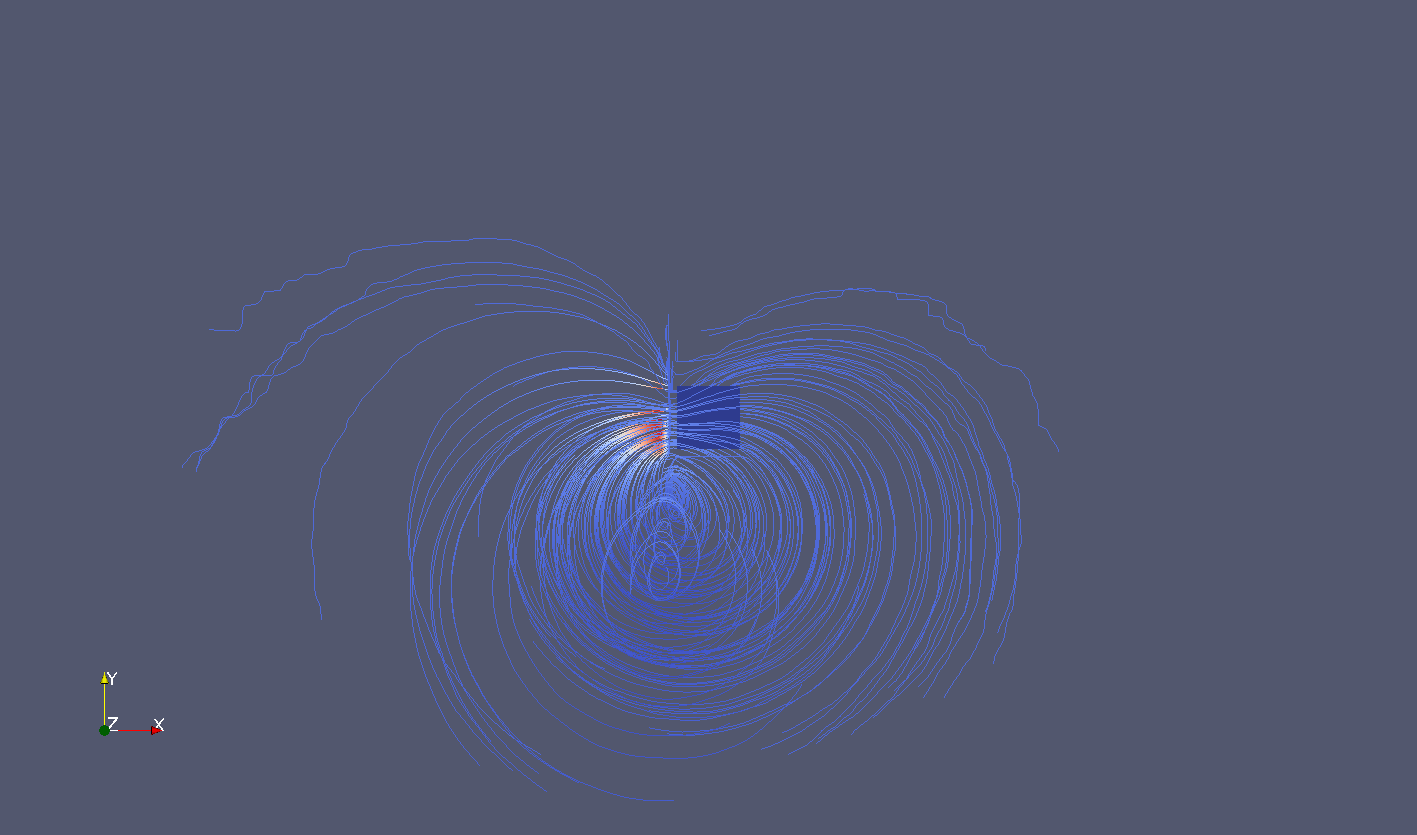
\includegraphics[width = 0.49 \textwidth]{images/case6_jph_paths}
		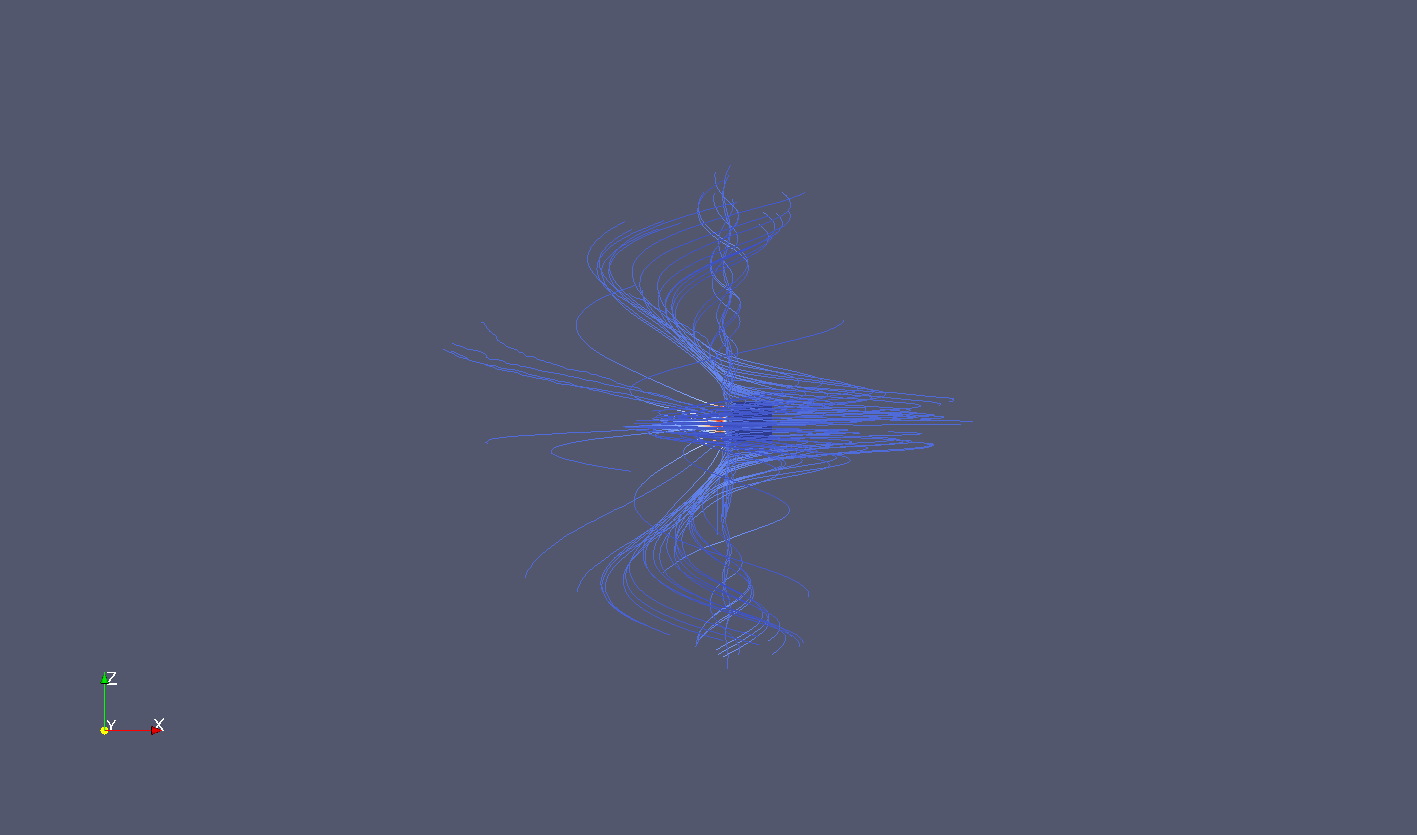
\includegraphics[width = 0.49 \textwidth]{images/case6_jph_paths_2}
		\caption{The trajectories of the electrons emmited by the photoelectric effect in simulation \(6\). It can be seen that some
		of the trajectories coincide with the volume occupied by the langmuir probes. The electrons are strongly affected by the magnetic
		field \(\vec{B}\), and follows a gyrating path.}
 	\end{figure}


\subsection{Potential difference with P-E and no P-E}

    \begin{figure}
        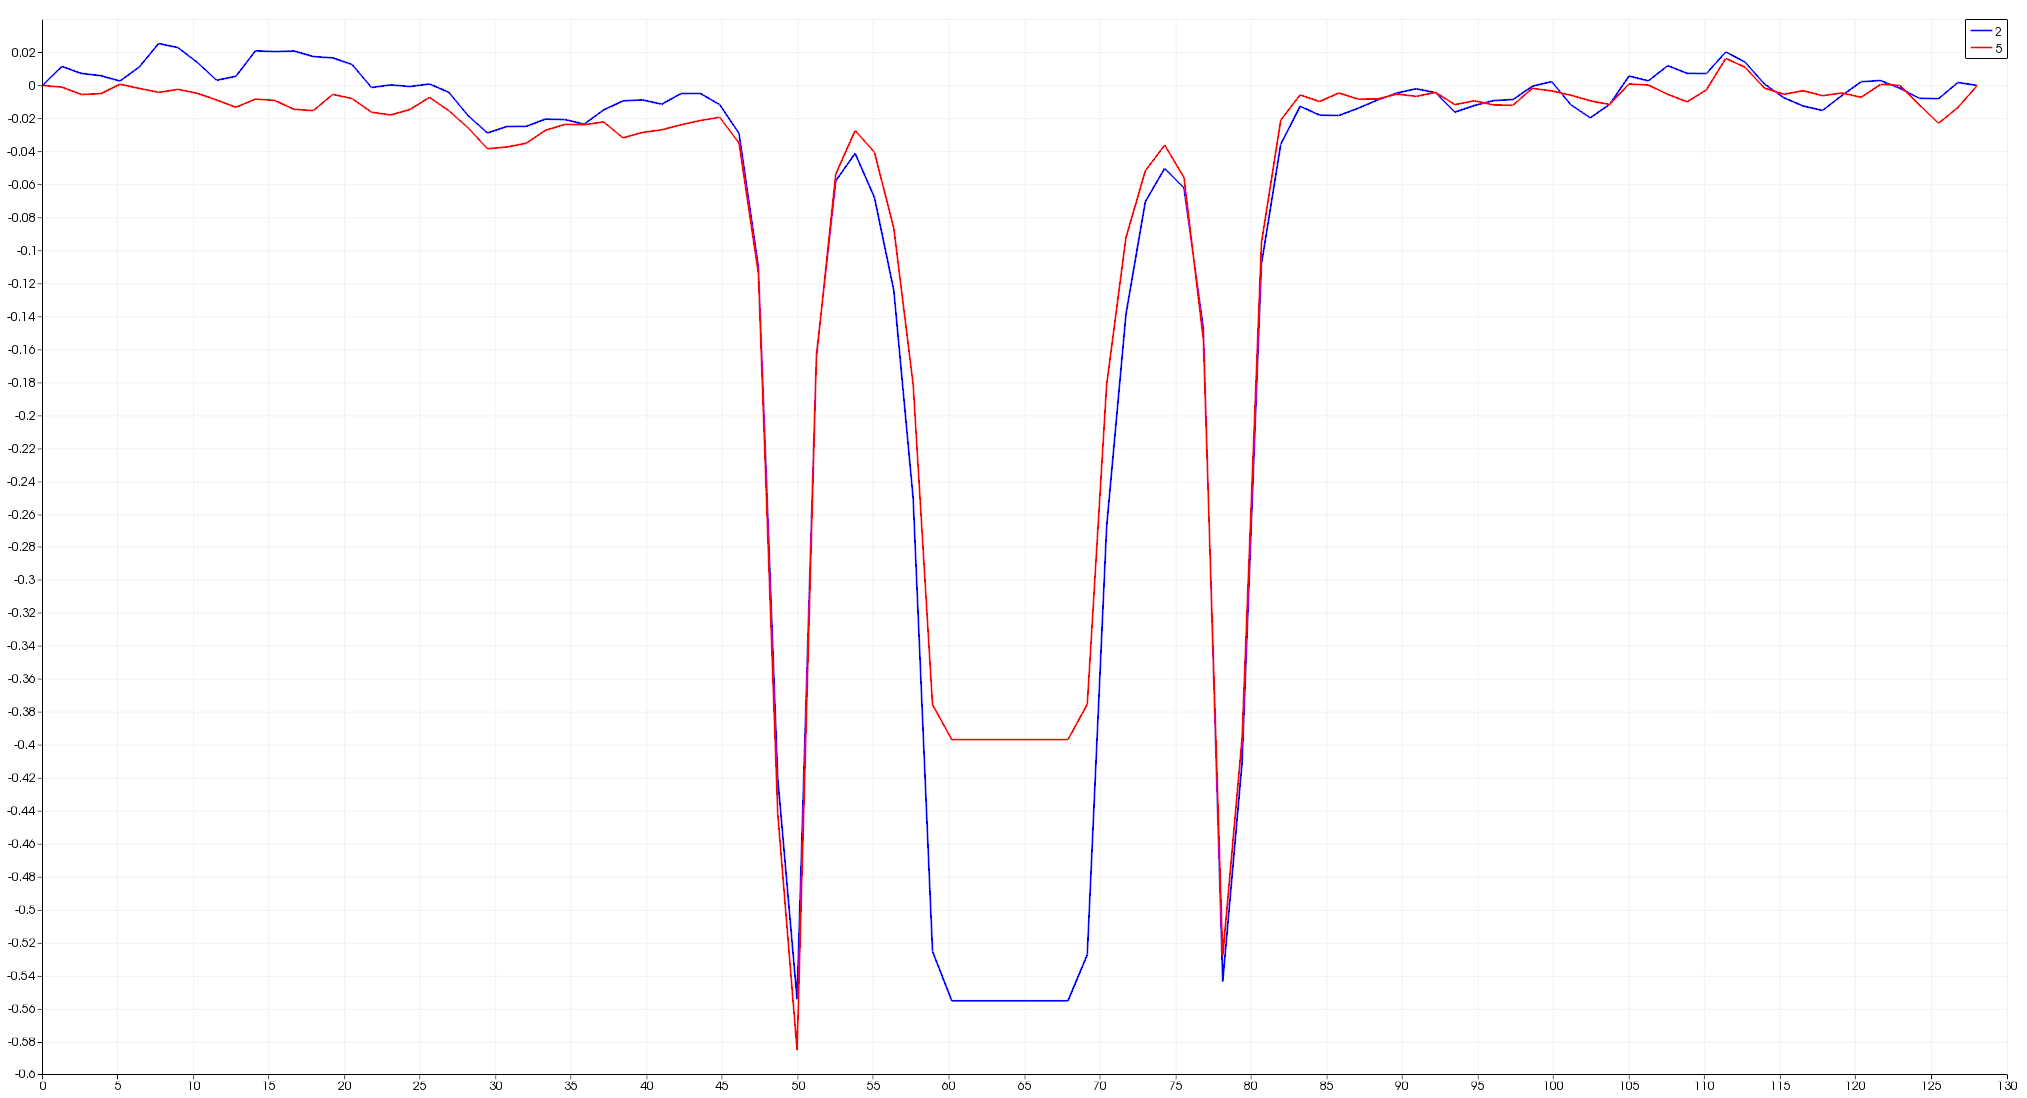
\includegraphics[width = 0.3 \textwidth]{images/pot_case25.png}
        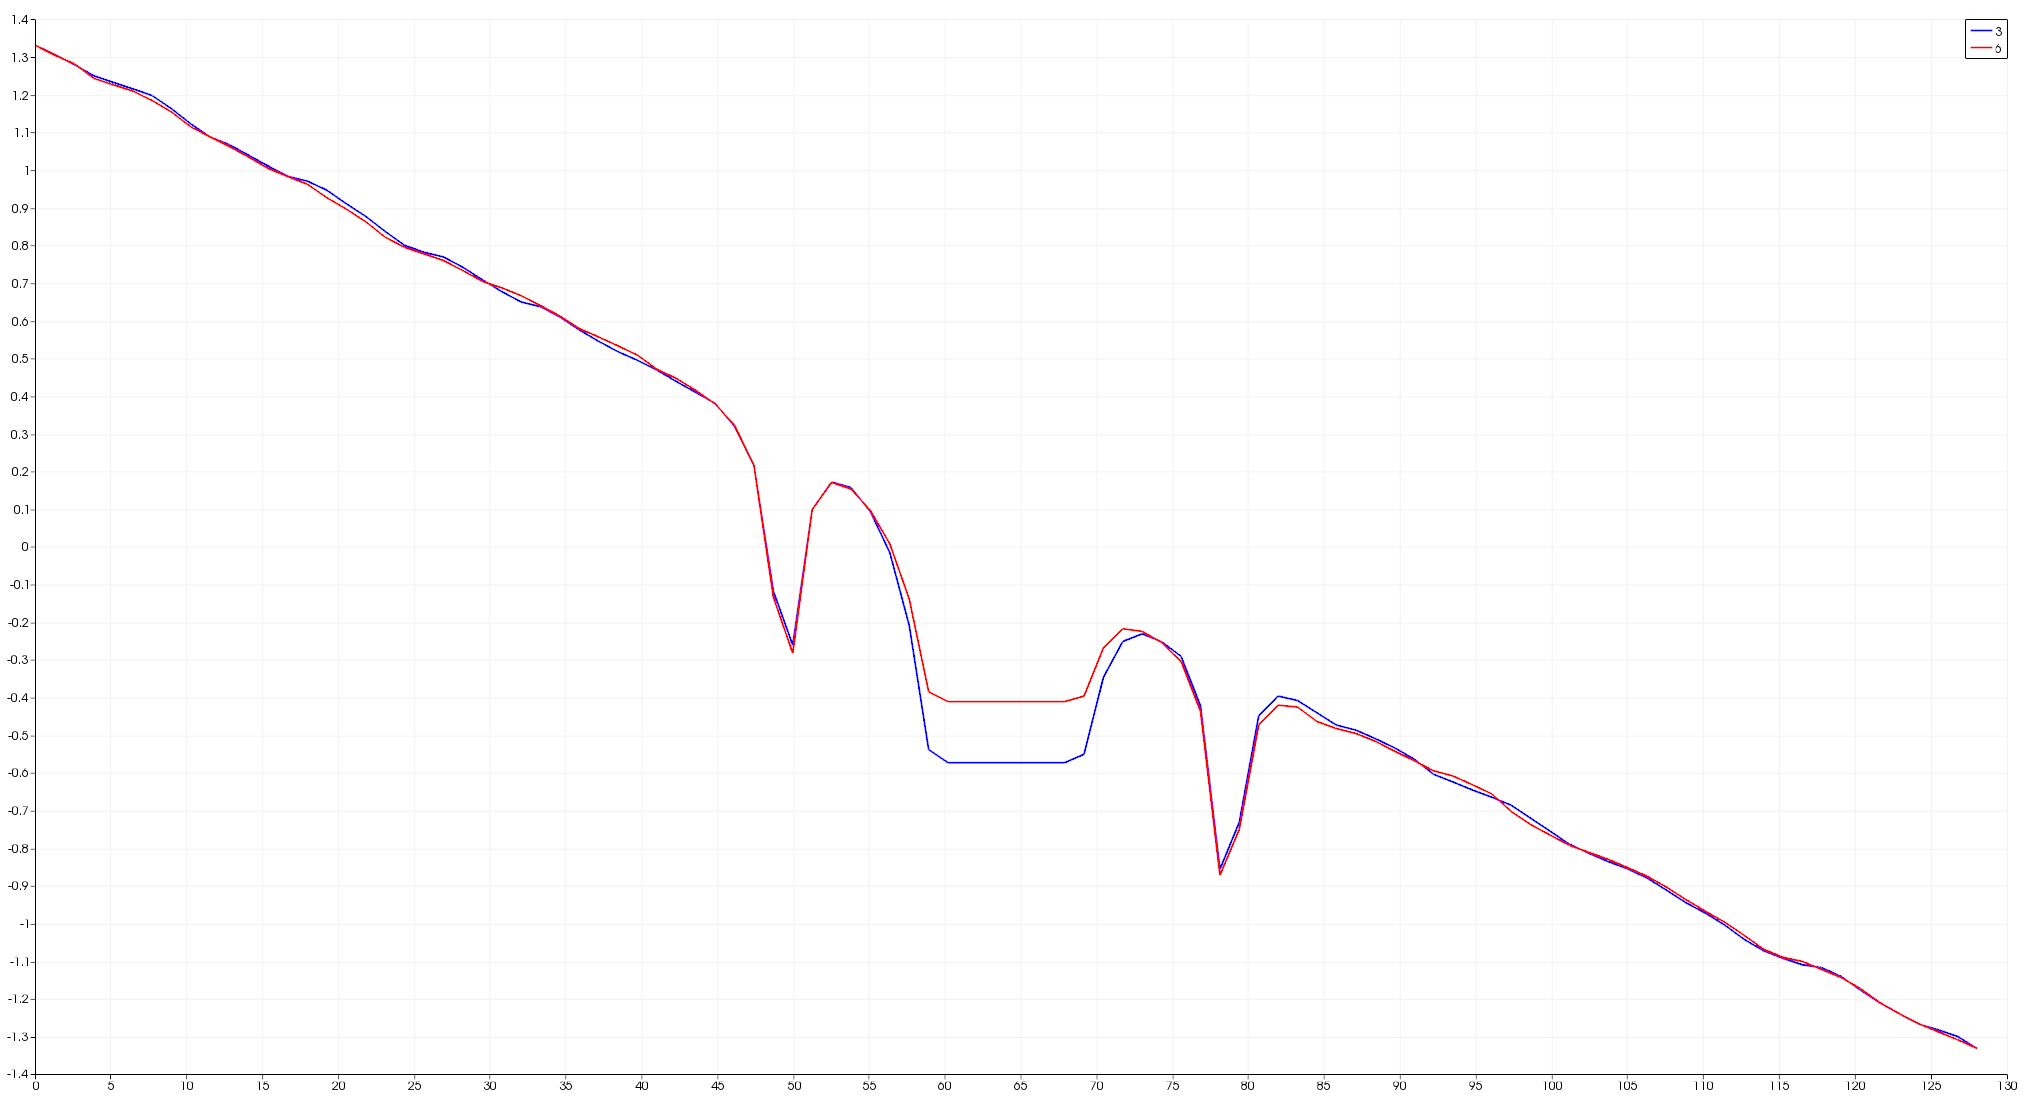
\includegraphics[width = 0.3 \textwidth]{images/pot_case36.png}
        \caption{Potential of spacecraft and surroundings with P-E and without P-E. Figure on the left displays difference between case 1 and 4. Middle figure displays difference between case 2 and 5. Rightmost figure displays difference between case 3 and 6.}
    \end{figure}
<<<<<<< HEAD


\subsubsection{Case 1 vs case 4}

Need plot 


\subsubsection{Case 2 vs case 5}

With the flow of emmited electrons in the negative x direction we would expect a rise in electron density around the left probe. This can be seen in the potential of this probe where there is a 5.4$%$ drop in the potential of this probe compared to no emitted electrons. On the right probe we have a small rise in potential of 3.3$%$. With no emitted electrons on this side of the satelite the rise in potential can be explained by looking at the increase in ion density as seen in figure (need ref). In the satelite we have a potential rise of 28$%$. So the change in potential in the probes are small compared to the change in the satelite.

\subsubsection{Case 3 vs case 6}

A rather large drop in potential of 12$%$ on both probes. Potential rise of 26$%$ over the satelite.  
    
=======
    
    
    
\subsection{Wake plots}
    
    \begin{figure}
        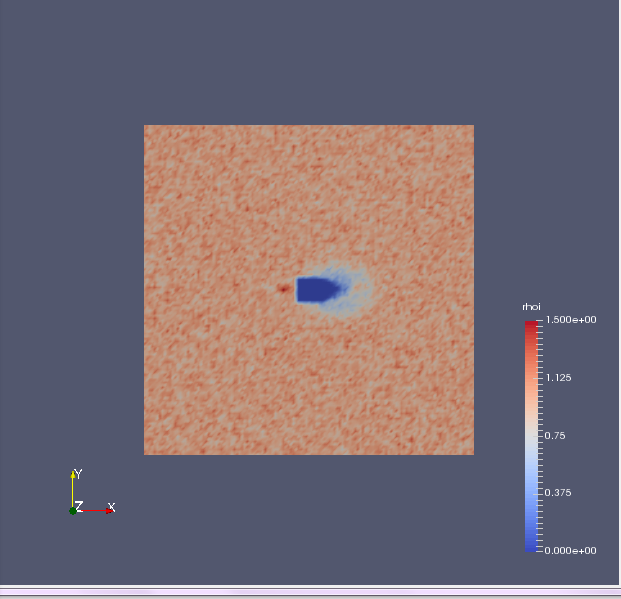
\includegraphics[width = 0.3 \textwidth]{images/ion density case1}
        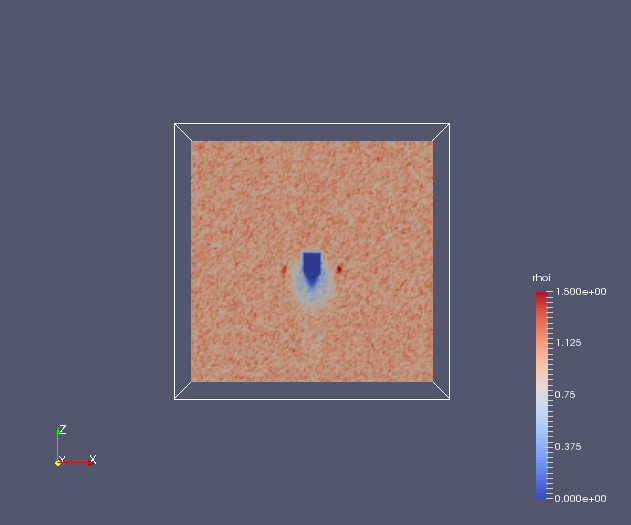
\includegraphics[width = 0.3 \textwidth]{images/ion density x-z case2}
	 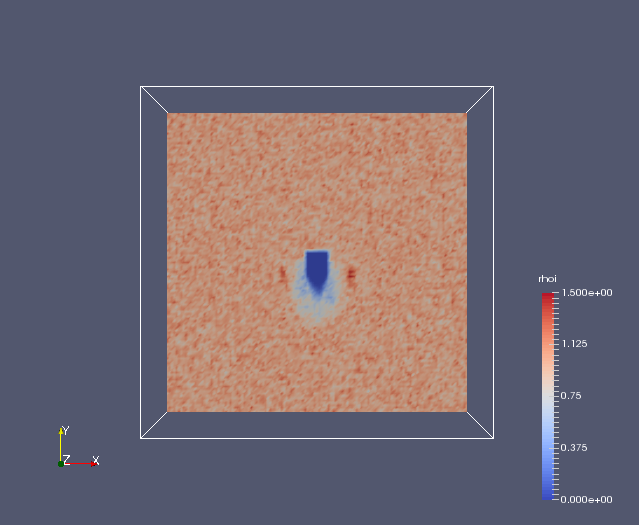
\includegraphics[width = 0.3 \textwidth]{images/ion density x-y case3}
        \caption{Ion density of spacecraft and surroundings without P-E. Figure on the left displays case 1. Middle figure displays case 2. Rightmost figure displays case 3.}
    \end{figure}
>>>>>>> 3b368f4c88efffdde9f90d1923ff1d456dc8f11c
